\section{透镜}\label{sec:1-6}

透镜是照相机、幻灯机等光学仪器的重要组成部分,通常是用玻璃磨成的。
它的一个侧面,或者两个侧面是球面的一部分。透镜可以分成两类:
一类是中央比边缘厚的,叫做\textbf{凸透镜},象图 \ref{fig:1-21} 里的 1、2、3;
另一类是中央比边缘薄的,叫做\textbf{凹透镜},象图 \ref{fig:1-21} 里的 4、5、6。

\begin{figure}[htbp]
    \centering
    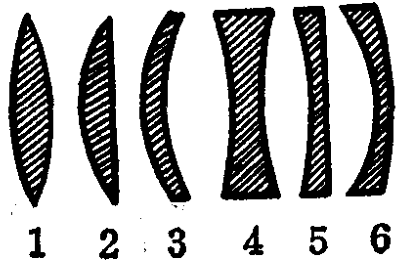
\includegraphics[width=0.3\textwidth]{../pic/czwl2-ch1-21}
    \caption{各种透镜}\label{fig:1-21}
\end{figure}

让一束平行光射在凸透镜上(图 \ref{fig:1-22}),可以看到,光通过凸透镜发生折射以后会聚于一点,
可见凸透镜对光有会聚作用,所以又叫做\textbf{会聚透镜}。

\begin{figure}[htbp]
    \centering
    \begin{minipage}{7cm}
    \centering
    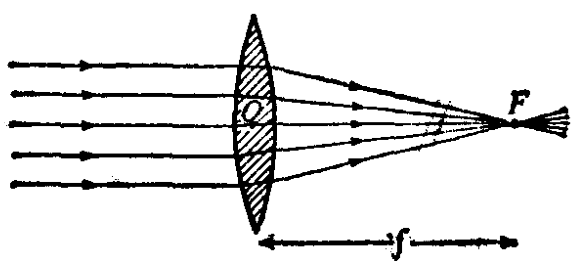
\includegraphics[width=6.5cm]{../pic/czwl2-ch1-22}
    \caption{凸透镜的会聚作用}\label{fig:1-22}
    \end{minipage}
    \qquad
    \begin{minipage}{7cm}
    \centering
    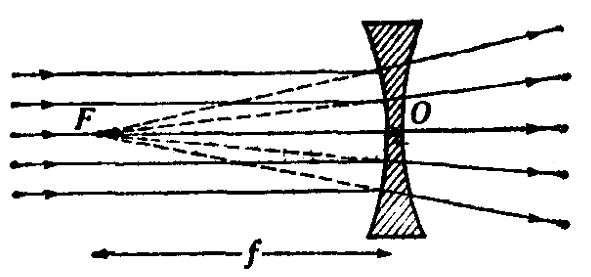
\includegraphics[width=6.5cm]{../pic/czwl2-ch1-23}
    \caption{凹透镜的发散作用}\label{fig:1-23}
    \end{minipage}
\end{figure}

让一束平行光射在凹透镜上(图 \ref{fig:1-23}),可以看到,光通过凹透镜发生折射以后向外散开。
可见凹透镜对光有发散作用,所以又叫做\textbf{发散透镜}。

\begin{figure}[htbp]
    \centering
    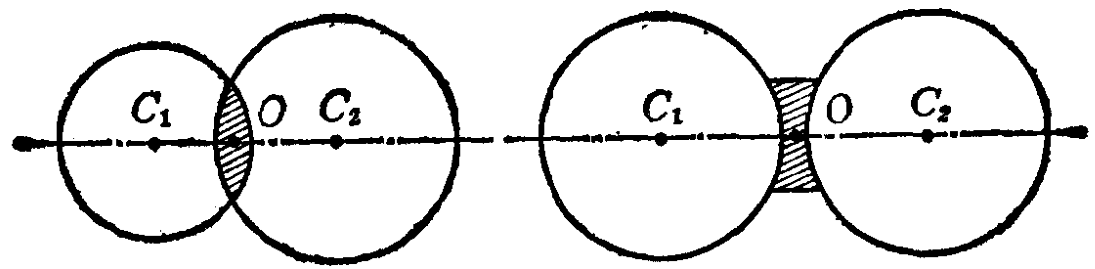
\includegraphics[width=0.7\textwidth]{../pic/czwl2-ch1-24}
    \caption{透镜的主轴}\label{fig:1-24}
\end{figure}

通过透镜两个球面的球心 $C_1$、$C_2$ 的直线,叫做透镜的\textbf{主轴}(图 \ref{fig:1-24})。
如果透镜的一个侧面是平面,透镜的主轴就跟这个平面垂直,并且通过另一侧面的球心。
通常用的透镜,厚度比球面的半径小得多,叫薄透镜。在中学里只研究薄透镜。

跟主轴平行的光通过凸透镜后会聚在主轴上的一点(图 \ref{fig:1-22} 中的 $F$),这个点叫做凸透镜的\textbf{焦点}。
跟主轴平行的光通过凹透镜后形成一个发散的圆锥(图 \ref{fig:1-23}),这些发散的光,
看起来象是从它们传播方向的反向延长线的交点 $F$ 发出来的,点 $F$ 也在主轴上,叫做凹透镜的焦点。
可见凹透镜的焦点不是光实际会聚点,所以是虚焦点,而凸透镜的焦点是光实际会聚点,所以是实焦点。
焦点到透镜中心 $O$ 的距离叫做\textbf{焦距},通常用 $f$ 表示。
透镜的两侧各有一个焦点,两个焦点到中心的距离相等。

\begin{wrapfigure}[11]{r}{7cm}
    \centering
    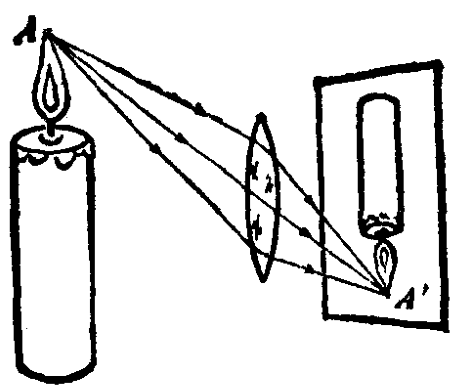
\includegraphics[width=6cm]{../pic/czwl2-ch1-25}
    \caption{光的折射}\label{fig:1-25}
\end{wrapfigure}

实验表明,如果把光源放在凸透镜的焦点上,光源发出的光通过凸透镜后一定平行射出。

凸透镜不但对光有会聚作用,而且还能够成像。

如图 \ref{fig:1-25} 所示,把凸透镜放在蜡烛和光屏的中间,调整它们的位置,可以在光屏上得到蜡烛的倒立像。
这个像是怎样形成的呢?我们先来考察顶端的一点 $A$。这一点发出的光向四周散射,其中一部分射到凸透镜上,
通过凸透镜的光线发生折射会聚于一点 $A'$,点 $A'$ 就是点 $A$ 的像。
同样,蜡烛上的每一点都产生一个像点。这许多像点组成了整个蜡烛的像。
这里,凸透镜所成的像是通过凸透镜的光实际会聚而成的,叫做\textbf{实像}。


